\section{Proposed Algorithm}
\label{sec:algorithm}


Our algorithm consists of two main parts:
a) \change{an} FCN-style network providing \change{initial} segmentation of the synaptic cleft;
b) a contour growing technique that uses the coarse segmentation as a start point to extract the whole contours.
The pipeline is illustrated in Fig.~\ref{fig:cg}.

\subsection{FCN segmentation}
%To accurately localize the location of target regions, an FCN-style network is first implemented to provide a coarse segmentation for synaptic cleft.
\change{The network architecture is} based on DeepLab (ResNet-101)~\cite{Chen2016a}, which uses the dilated convolution for lager receptive fields.
%
We also explore \change{different network architectures in our framework and the results demonstrate the robustness of our model in Sec.~\ref{sec:experiments}.}
%
For the synaptic cleft segmentation, we modify the classifier of DeepLab to a binary classifier and use a weighted loss for mitigating the unbalanced label problem in our task.
For the problem of limited data caused by the expensive acquisition, the transfer learning strategy is used by fine-tuning the weights of lower layers on the off-the-shelf model from DeepLab, which have been well trained on natural images.

\xj{What happens if there are multiple cleft regions?}

\subsection{Contour growing}

Based on the binary mask from \change{FCN} segmentation, we first generate an initial centric curve, which will be evolved to respectively attach to presynaptic and postsynaptical membranes.
%
\change{More specifically}, the initial centric curve is obtained by \change{fitting a quadratic spline on all the positive pixels in the mask and truncating the middle part in a small length.}
%truncating a quadratic curve fitted on the positive pixels of the mask.
%
In order to make sure that the initial centric curve is inside the cleft region, it will be generated as short as possible, such as the green dotted line in Fig.~\ref{fig:cg}.
%
\change{The initial centric curve is first evolved on the two opposite directions to 
	find the contours of both the presynaptic and postsynaptical membranes.}
Then the contours at the two sides are extended synchronously to extract the whole synaptic cleft region.




\subsubsection{Curve evolving}
\label{sec:curve_evolving}


Similar to the traditional snake model~\cite{Kass1988}, the initial centric curve is expressed by a parameterized model $\mathbf{v}(s)=\big(x(s),y(s)\big)$, where $s\in[0,1]$ is the arc-length along the curve.
Our goal is to minimize the following energy function:
\begin{eqnarray}\label{Eq:Etotal}
E_{total} =&\int_{0}^{1} E_{int}\big( \vb{v}(s) \big)+ E_{ext}\big( \mathbf{v}(s)\big) ds\nonumber \\
E_{int} = & \alpha|\mathbf{v}^{'}(s)|+\beta|\mathbf{v}^{''}(s)| \\\nonumber
E_{ext} =& I\big( \mathbf{v}(s)\big) + \kappa G\big(\mathbf{v}(s)\big),\nonumber
\end{eqnarray}
where $\mathbf{v}^{'}(s)$ and $\mathbf{v}^{''}(s)$ are the first-order and second-order derivatives of $\mathbf{v}(s)$, controlling the curve to be smooth and straight.
$E_{ext}$ consists of a Gaussian smoothed image $I$ and a gradient magnitude map $G$, which drive the curve to the edge region with dark pixel value.  
According to \cite{Kass1988}, Eq.~\ref{Eq:Etotal} can be minimized by iteratively updating the following equation:
\begin{eqnarray}\label{Eq:GVF}
V_{t+1} = (\vb{A}+\gamma \vb{I})^{-1}(\gamma V_t+\mathbf{f}(V_t)),
\end{eqnarray}
where $V\in R^{np\times2}$ and $np$ is the number of discrete controlling points of $\mathbf{v}(s)$.
$\vb{A}$ is a matrix encoding the internal tension, $\gamma$ controls the evolving rate and $\mathbf{f}=[f_{x},f_{y}]$ are the gradient maps calculated from $E_{ext}$ using Gradient Vector Flow (GVF) algorithm \cite{Xu1998}.

\begin{figure}[t]
	\begin{center}
		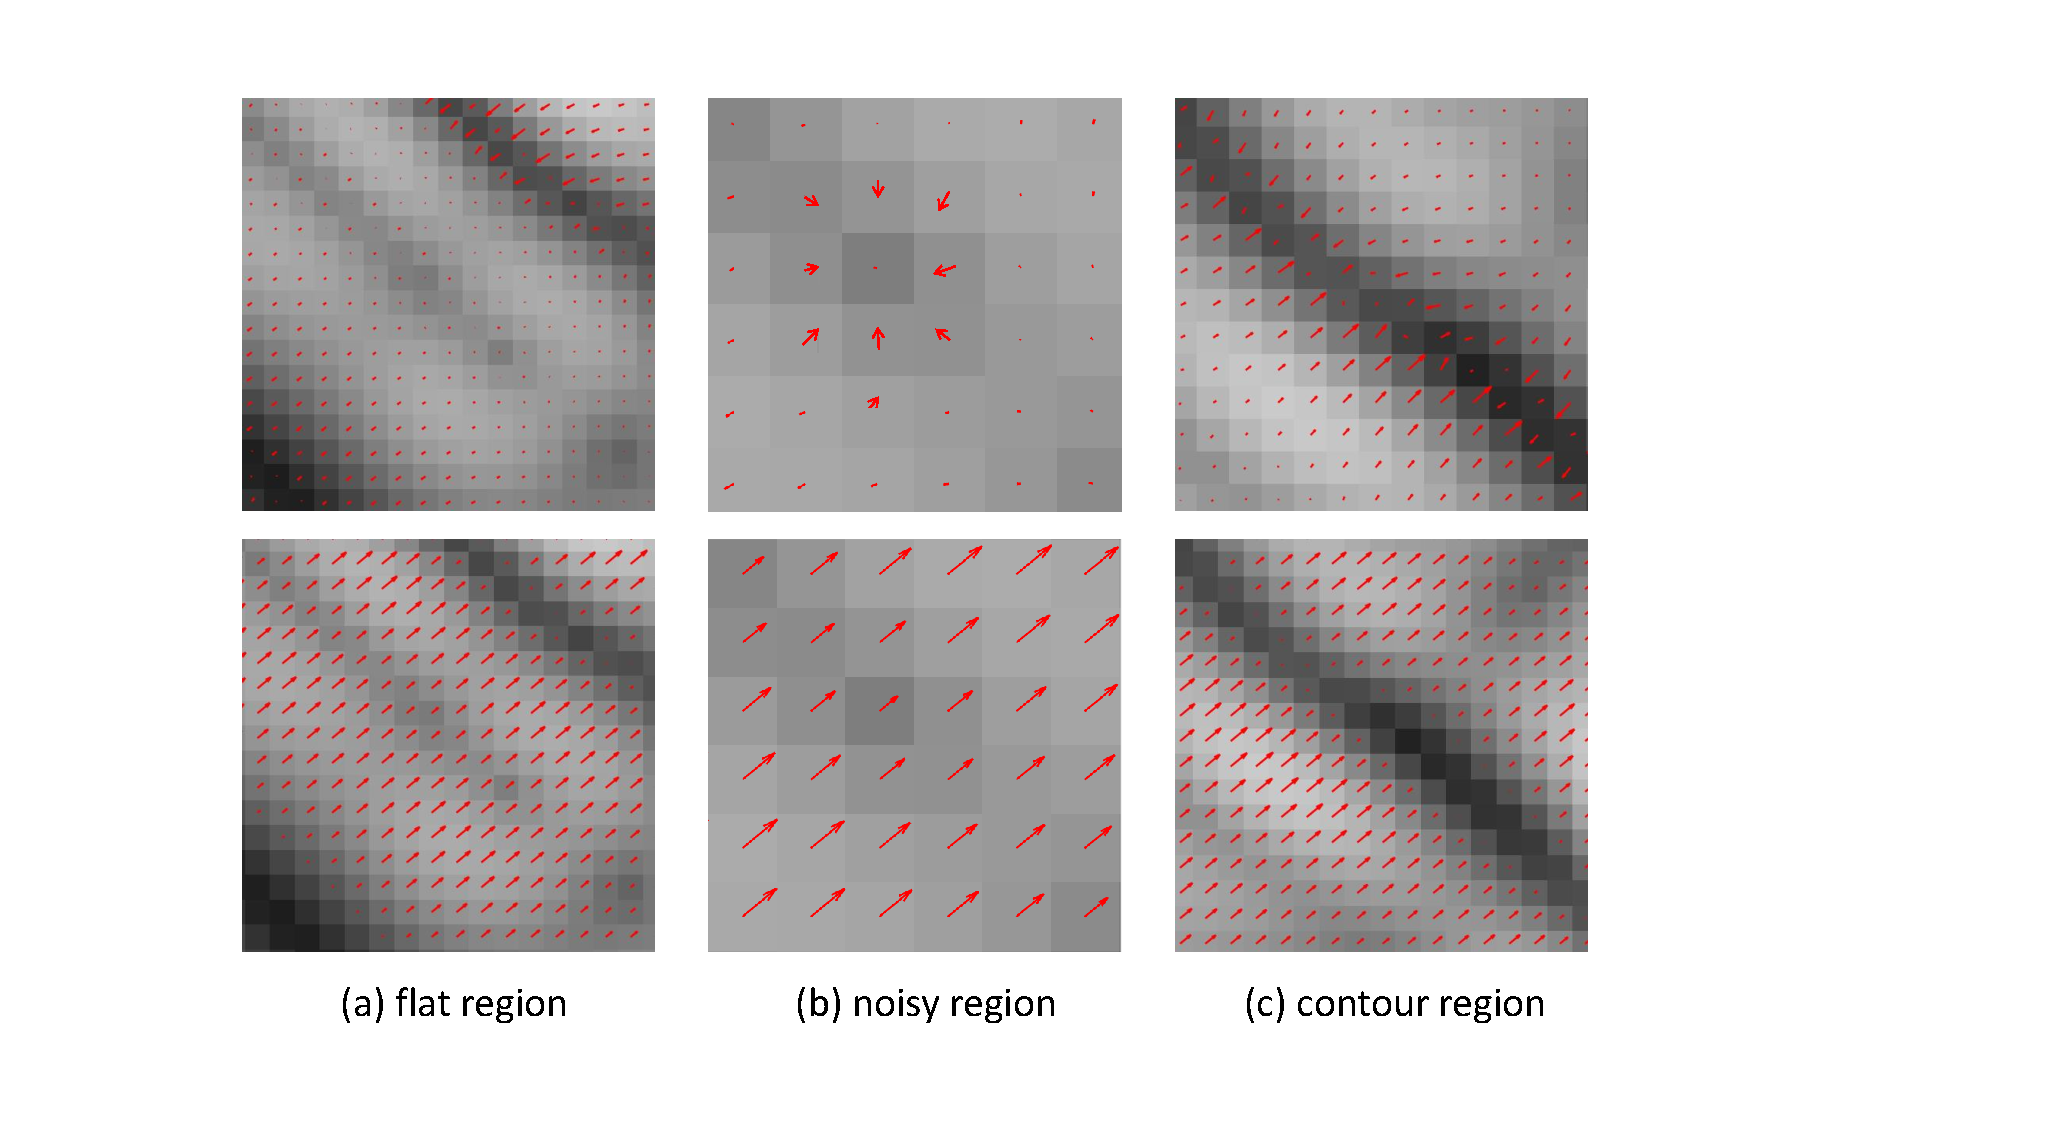
\includegraphics[width=3.4in]{figs/FigGVF.pdf}
	\end{center}
	%
	\caption{Several cases of tension field obtained by GVF (top row) and our normal force (bottom row). The red arrow indicates the force vector of external tension.}
	\label{fig:gvf}
\end{figure}

However the updating strategy of Eq.~\ref{Eq:GVF} is not robust in our electron micrographs with high noise.
Firstly, in some flat regions with small gradients $\mathbf{f}$, the external tension is too weak to drive the controlling points $V_{np}$ to move against to internal tension.
Therefore, it requires the initial curve to be away from the flat regions.
Secondly, the external tension in some noisy regions will be gyrate, which easily trap some control points.
Although sometimes the internal tension may pull the trapped points out, the gyrate $\mathbf{f}$ will trap them again.
Thirdly, as the gradients $\mathbf{f}$ near to contours are usually large, $V_{np}$ easily cross the optimal positions by over-huge tension,
Top row cases of Fig.~\ref{fig:gvf} represents the above discussion.
Thus in this section, we propose a new updating strategy by:
\begin{eqnarray}\label{Eq:update}
V_{t+1} = (A+\gamma I)^{-1}(\gamma V_t+E_{ext}(V_t)N)
\end{eqnarray}
$N\in R^{np\times2}$ consists of the normal vectors of $np$ controlling points with consistent orientations.

In Eq.~\ref{Eq:update}, the moving direction of each $V_{np}$ drove by external tension is fixed as its normal direction $N_{np}$, whose magnitude is $E_{ext}(V_{np})$ rather than a constant value in Ballons model \cite{Cohen1991}.
The advantages of Eq.~\ref{Eq:update} are follows:
a) the capture range of external tension are much larger, due to fixed external tension $E_{ext}(V)N$;
b) once $V_{np}$ is pulled away from the noisy region, $E_{ext}(V_{np})N_{np}$ will soon push it away.
c) our external tension will soon vanish in contour region due to small $E_{ext}$, which makes the updating more robust.
Bottom row cases of Fig.~\ref{fig:gvf} show our superiority over GVF.

By setting \change{two} opposite normal vectors ($\mathbf{n}_{+}$ and $\mathbf{n}_{-}$ in Figure~\ref{fig:cg}), \change{the centric curve} will be evolved along two opposite directions and well attach to the presynaptic and postsynaptical membranes.
The final evolved curves are respectively denoted as $\mathbf{c}_1(s)$ and $\mathbf{c}_2(s)$.

\begin{figure}[t]
\begin{minipage}[b]{1.0\linewidth}
  \centering
 \centerline{\epsfig{figure=Figs/FigG.pdf,width=8.5cm}}
\end{minipage}
\caption{The contour growing process formulated by Eq.~\ref{Eq:sg}.
        The yellow solid arrow indicates the growing direction of previous stages. The dotted arrows are the candidates of growing direction. The longest arrow is the selected growing contour.}
\label{fig:g}
\end{figure}

\subsubsection{Synchronous growing}

With the two initial pieces of contour $\mathbf{c}_1(s)$ and $\mathbf{c}_2(s)$, we then grow them to localize the whole \change{cleft region}.
The challenge of this part is that they should be grown correctly and synchronously to compute the exact distance between two membranes for termination judging.

First, we formulate the process of growing a contour $\mathbf{c}_(s)$ as iteratively finding a piece of straight line segment with length $l$ and unit vector $\mathbf{v}_l$:
\begin{eqnarray}\label{Eq:sg}
&\arg\min\limits_{l,\mathbf{v}_l} \sum\limits_{i=0}^{l}E_{int}(i\mathbf{v}_l+\mathbf{q}) -\rho\|\mathbf{v}_q \cdot \mathbf{v}_l\|,\\
&st.~ |\mathbf{v}_q \cdot \mathbf{v}_l| \leq \tau, \nonumber
\end{eqnarray}
where $\mathbf{q}$ is the current endpoint of $\mathbf{c}(s)$, and $\mathbf{v}_{q}$ is the tangent vector of $\mathbf{q}$ on the curve.
%
Similarly, we use $l$ points to represent the target straight line length for convenience.
The firs term of Eq.~\ref{Eq:sg} expects $\mathbf{c}_(s)$ to grow along the membranes with low \change{$E_{ext}$}, while the second term \change{prefers the growing direction following the previous direction of the contour}.
$\rho$ is a tradeoff parameter, and $\tau$ add a hard \change{constraint} on the growing direction to be not changed too much.
%
Optimal solution of Eq.~\ref{Eq:sg} can be obtained by alternatively updating $l$ and $\vb{v}_l$.
First, we fixed $l$ as a small value ($5$ pixels), to find the optimal $\vb{v}_l$, and then fix $\vb{v}_l$ to find a better $l$.
Experiments show that two iterations are good enough for most cases to generate a satisfying piece of new growing membrane, as shown in Fig.~\ref{fig:g}.

To synchronously grow $\mathbf{c}_1(s)$ and $\mathbf{c}_2(s)$, we split the growing process into several periods and decide which curve grows in each period.
%
Especially, we set two variables $g_1^{t+1}$ and $g_2^{t+1}$  ($1$ for growing and $0$ for waiting) to determine the growing state of $\mathbf{c}_1^{t}(s)$ and $\mathbf{c}_2^{t}(s)$ at stage $t+1$ by:
\begin{eqnarray}\label{Eq:gf}
g_1^{t+1},g_2^{t+1} = \left\{\begin{array}{cc}
0,1&if~(\mathbf{e}_1^t-\mathbf{e}_2^t)(\mathbf{e}_3^t-\mathbf{e}_2^t)^{T}\geq 0 \\
1,0&if~(\mathbf{e}_2^t-\mathbf{e}_1^t)(\mathbf{e}_3^t-\mathbf{e}_1^t)^{T}\geq 0\\
1,1& else\\
\end{array}\right.
\end{eqnarray}
where $\mathbf{e}_1^t$, $\mathbf{e}_2^t$ and $\mathbf{e}_3^t$ are the three endpoints of two membranes of stage $t$.
Different situations of Eq.~\ref{Eq:gf} are shown in Fig.~\ref{fig:sg}.
The distance between two membranes is calculated by:
\begin{eqnarray}\label{Eq:d}
d^{t+1} = \frac{||\mathbf{e}_1^{t+1}-\mathbf{e}_3^{t+1}||+ ||\mathbf{e}_1^{t}-\mathbf{e}_3^{t}||}{2}.
\end{eqnarray}
Once $d^{t+1}$ is beyond the range of \change{a} reasonable cleft width, the \change{growth is} terminated.
\begin{figure}[t]
\begin{minipage}[b]{1.0\linewidth}
  \centering
 \centerline{\epsfig{figure=Figs/FigSG.pdf,width=8.5cm}}
\end{minipage}
\caption{Diagram of different situations illustrated in Eq.~\ref{Eq:gf}.
        The green lines are the new growing contour, while the red lines are the previous contours}
\label{fig:sg}
\end{figure}
